\section{Digital Images}
Digital images consists of a discrete number of discrete valued data points called pixels. It is the value of these pixels that determine their color. A pixel's value is also called its \emph{intensity} and will lie within a range of values determined by the image's encoding. For example an 8-bit image has pixel values in the range $[0, 255]$. 

Digital images are often represented as a 2D array of values where each cell corresponds to an intesnity. In software in particular,  digital images are stored and manipulated as arrays. An image's array is $M\times N$ pixels in size, which is also its resolution. Notice that in Figure \ref{fig:2Darray} the lowest value is 0 (black) and the highest value is 255 (white). All other colors that can be represented by 8-bits are between these two values.

\begin{figure}[H]
    \centering
    \begin{subfigure}[b]{0.5\linewidth}
      \centering
\includegraphics[width=150pt]{chessboard}
      \caption{\label{fig:fig1}}
    \end{subfigure}%
    \begin{subfigure}[b]{0.5\linewidth}
      \centering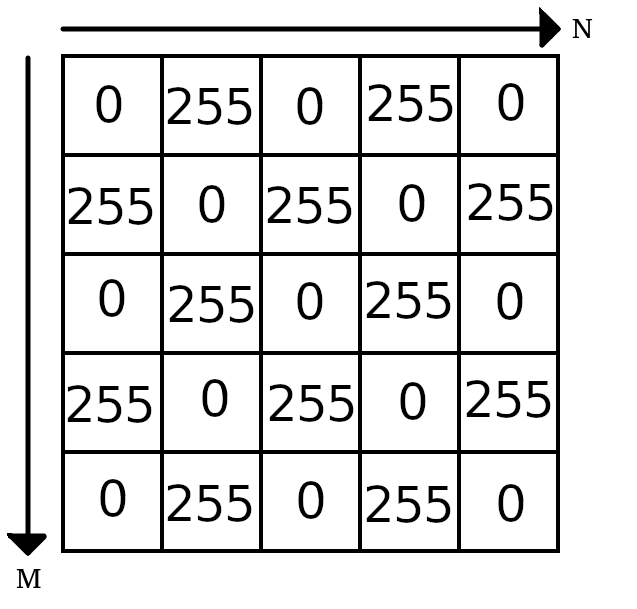
\includegraphics[width=150pt]{array2}
      \caption{\label{fig:fig2}}
    \end{subfigure}
    \caption{(\subref{fig:fig1}) A Simple 8-bit Image ~(\subref{fig:fig2}) Array Representation of Image.}
    \label{fig:2Darray}
\end{figure}
  

2D array representation allows pixels to be referenced by their relative position in the $M$ and $N$ directions. Furthermore, $M$ and $N$ may be substituted for the x and y axes of the Cartesian plane. In fact, a digital image is just a two dimensional function where each pixel is described by a coordinate (x,y) and an intensity (z) at that point.

\begin{equation}
    z = f(x,y)
    \label{eq:2Dfunc}
\end{equation}

This means that two dimnesional operations may be applied to a digital image and images may be modelled as 3D surfaces. Modelling images as a surface is useful when trying to visualize rates of change in an image. In Figure \ref{fig:2Darray} you can see that there is a rapid change in value between different coloured squares, shown as steep cliff edges.

\begin{figure}[ht!]
  \centering
  \centering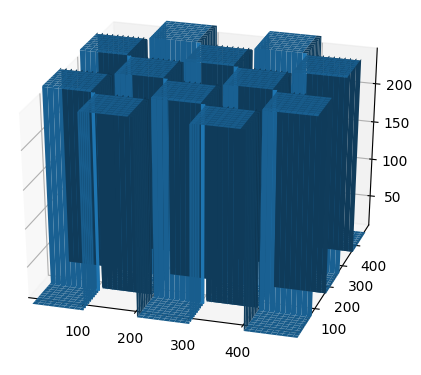
\includegraphics[width=150pt]{3Dchess}
  \caption{\label{fig:fig1} Surface Plot of Figure \ref{fig:2Darray}\ref{sub@fig:fig1}}
\end{figure}




